\documentclass[a4paper]{article}
\usepackage[utf8]{inputenc}
\usepackage{polski}
\usepackage[T1]{fontenc}
\usepackage{amsmath,amssymb,amsthm}
\usepackage{lmodern}
\usepackage[a4paper]{geometry}
\usepackage[dvipsnames]{xcolor}
\usepackage{hyperref}
\usepackage{array}
\usepackage{caption}
\usepackage{tikz}
\usepackage{pgfplots}
\pgfplotsset{compat=1.15}
\usepackage{mathrsfs}
\usetikzlibrary{arrows}

\definecolor{ududff}{rgb}{0.30196078431372547,0.30196078431372547,1.}
\definecolor{xdxdff}{rgb}{0.49019607843137253,0.49019607843137253,1.}
\definecolor{uuuuuu}{rgb}{0.26666666666666666,0.26666666666666666,0.26666666666666666}


% do uzupełnienia
\newcommand{\todo}[1]{\begin{center} \fbox{TODO: #1} \end{center}}

% wyłączenie wcięć
\setlength\parindent{0pt}

% matematyczne
\renewcommand{\mod}{\,\, \text{mod} \,\,}
\newcommand{\shift}[2]{\text{shift}_{#2}^{#1}}
\newcommand{\sym}[2]{\text{sym}_{#2}^{#1}}
\newcommand{\id}[1]{\text{id}_{#1}}
\newcommand{\td}{\text{.}}
\newcommand{\tc}{\text{, }}
\newcommand{\floor}[1]{\left\lfloor #1 \right\rfloor}
\newcommand{\twoshift}[1]{\text{TwoShift}_{#1}}
\newcommand{\N}{\mathbb{N}}
\newcommand{\lt}{\left}
\newcommand{\rt}{\right}
\newcommand{\R}{\mathbb{R}}

% twierdzenia, lematy, definicje, fakty, wnioski
\newtheorem{tw}{Twierdzenie}[section]
\newtheorem{lem}[tw]{Lemat}
\theoremstyle{definition}
\newtheorem{df}[tw]{Definicja}
\newtheorem{wn}[tw]{Wniosek}
\newtheorem{fa}[tw]{Fakt}
\newtheorem*{pyt}{Pytanie}

\begin{document}

% ---------- strona tytułowa -----------------

\newpage
\thispagestyle{empty}
\begin{center}
\textbf{\large Uniwersytet Wrocławski\\
Wydział Matematyki i Informatyki\\
Instytut Matematyczny}\\
% \textit{\large specjalność: wpisz tu specjalność}\\
\vspace{4cm}
\textbf{\textit{\large Maksymilian Adamczewski i Jadwiga Świerczyńska}\\
\vspace{0.5cm}
{\Large Sieci przełączników}}\\
\end{center}
\vspace{3cm}
{\large \hspace*{6.5cm}Praca zespołowa\\
\hspace*{6.5cm}napisana pod opieką\\
\hspace*{6.5cm}dr. hab. Jana Dymary, prof. UWr }\\
\vfill
\begin{center}
{\large Wrocław, 2023 r.}\\
\end{center}

% -------------- abstrakt ----------------------

\newpage

\null\vfill

\begin{abstract}
    \todo{streszczenie}
    % Sieci przełączników bla bla bla
\end{abstract}

\vfill


% -------------- spis treści --------------------

\newpage

\tableofcontents

\newpage


% -------------- wprowadzenie --------------------

\section{Wprowadzenie}

Sieci przełączników to struktury, które można zinterpretować jako urządzenia zbudowane z tzw. \textit{przełączników} pozwalające na permutowanie \(n\) rozróżnialnych sygnałów danych na wejściu. Naturalne jest, że dążymy do optymalizacji struktury sieci pod względem liczby użytych przełączników lub maksymalnej liczby przełączników, przez jakie przepływa sygnał w sieci. Jednakże ze względu na wysoce wyspecjalizowane zastosowania (m. in. sieci telefoniczne, trasowanie pakietów) brakuje źródeł wyczerpująco tłumaczących to zagadnienie w sposób przystępny na przykład dla studenta drugiego roku informatyki. W tej pracy przybliżymy podstawowe definicje (rozdział 2), przedstawimy konstrukcję najsłynniejszej sieci realizującej wszystkie permutacje, czyli sieci Beneša--Waksmana (rozdział 3), sieci realizującej wszystkie przesunięcia cykliczne (rozdział 4) i sieci realizującej przesunięcia cykliczne o potęgi 2 (rozdział 5).  Natomiast w rozdziale 6 przeanalizujemy sieci, w których przełączniki są ustawiane losowo w jeden z dwóch stanów. 

\vspace{1em}

Zastrzegamy jednak, że za względu na cel pracy, polegający na przystępnym przybliżeniu tematu, przy formułowaniu definicji i konstrukcji będziemy skupiać się na intuicji. Precyzyjną matematyczną formalizację pozostawimy jako ćwiczenie dla Czytelnika, które okaże się schematycznym zadaniem, gdy już się zrozumie idee stojące za sieciami przęłączników. 

\vspace{1em}

Przez \(S_n\) będziemy oznaczać zbiór wszystkich permutacji \(\{0, 1, \ldots, n-1\}\), przez
\[
\shift{n}{k} : \{0, 1, \ldots, n-1\} \to \{0, 1, \ldots, n-1\} 
\]
permutację \(\shift{n}{k}(i) = (k+i) \mod n\), a przez
\[
\sym{n}{k} : \{0, 1, \ldots, n-1\} \to \{0, 1, \ldots, n-1\} 
\]
permutację \(\sym{n}{k}(i) = (k-i) \mod n\), natomiast przez 
\[
\id{n} : \{0, 1, \ldots, n-1\} \to \{0, 1, \ldots, n-1\} 
\]
permutację identycznościową. 

\todo{definicje notacji asymptotycznej}


% -------- podstawowe definicje i fakty -----------

\section{Podstawy}

\subsection{Definicje}

Zacznijmy od najistotniejszej dla tej pracy kwestii -- czyli definicji przełącznika.

\vspace{1em}

{\bf Przełącznikiem} nazywamy urządzenie mające dwa wejścia (oznaczone liczbami 0 i 1)  i dwa wyjścia (oznaczone liczbami 0 i 1). Może się znaleźć w dwóch stanach:

\begin{itemize}
    \item nieaktywnym -- sygnał z wejścia \(i\) trafia do wyjścia \(i\) (dla \(i \in \{0,1\}\)),
    \item  aktywnym -- sygnał z wejścia \(i\) trafia do wyjścia \((i+1) \mod 2\) (dla \(i \in \{0,1\}\)).
\end{itemize}

\todo{rysunek przełącznika w dwóch stanach}
\begin{center}
    \begin{minipage}{.5\textwidth} %
        \begin{center}
            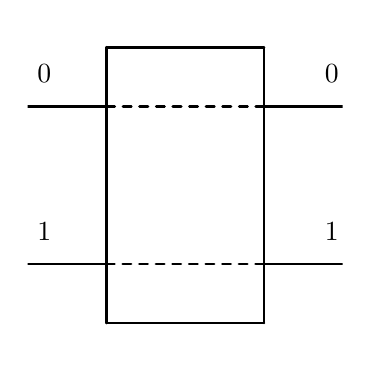
\begin{tikzpicture}[line cap=round,line join=round,>=triangle 45,x=0.5cm,y=0.5cm]
            \clip(-2,-1.) rectangle (6.,7.5);
            \draw [line width=1.pt] (0.,0.)-- (4.,0.);
            \draw [line width=1.pt] (4.,0.)-- (4.,7.);
            \draw [line width=1.pt] (4.,7.)-- (0.,7.);
            \draw [line width=1.pt] (0.,7.)-- (0.,0.);
            \draw (-2.,6.8) node[anchor=north west] {0};
            \draw (5.3,6.8) node[anchor=north west] {0};
            \draw (-2.,2.8) node[anchor=north west] {1};
            \draw (5.3,2.8) node[anchor=north west] {1};
            \draw [line width=1.pt] (0.,5.5)-- (-2.,5.5);
            \draw [line width=1.pt] (4.,5.5)-- (6.,5.5);
            \draw [line width=1.pt] (0.,1.5)-- (-2.,1.5);
            \draw [line width=1.pt] (4.,1.5)-- (6.,1.5);
            \draw [line width=1.pt, dashed] (4.,1.5)-- (0.,1.5);
            \draw [line width=1.pt, dashed] (0.,5.5)-- (4.,5.5);
            \end{tikzpicture}
            
            {\it Przełącznik w stanie nieaktywnym}
        \end{center}
        
    \end{minipage}%
    \begin{minipage}{.5\textwidth} %
        \begin{center} 
            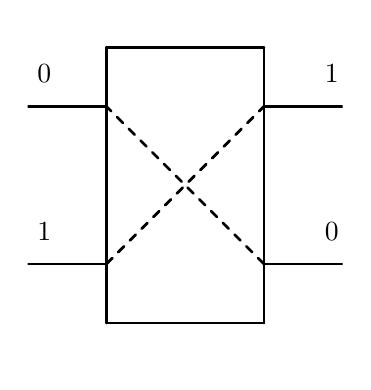
\begin{tikzpicture}[line cap=round,line join=round,>=triangle 45,x=0.5cm,y=0.5cm]
            \clip(-2,-1.) rectangle (6.,7.5);
            \draw [line width=1.pt] (0.,0.)-- (4.,0.);
            \draw [line width=1.pt] (4.,0.)-- (4.,7.);
            \draw [line width=1.pt] (4.,7.)-- (0.,7.);
            \draw [line width=1.pt] (0.,7.)-- (0.,0.);
            \draw (-2.,6.8) node[anchor=north west] {0};
            \draw (5.3,6.8) node[anchor=north west] {1};
            \draw (-2.,2.8) node[anchor=north west] {1};
            \draw (5.3,2.8) node[anchor=north west] {0};
            \draw [line width=1.pt] (0.,5.5)-- (-2.,5.5);
            \draw [line width=1.pt] (4.,5.5)-- (6.,5.5);
            \draw [line width=1.pt] (0.,1.5)-- (-2.,1.5);
            \draw [line width=1.pt] (4.,1.5)-- (6.,1.5);
            \draw [line width=1.pt, dashed] (4.,1.5)-- (0.,5.5);
            \draw [line width=1.pt, dashed] (0.,1.5)-- (4.,5.5);
            \end{tikzpicture}

            {\it Przełącznik w stanie aktywnym}
        \end{center}
    \end{minipage} 
\end{center}

\vspace{1em}

Przełączniki w naturalny sposób możemy ze sobą łączyć {\bf przewodami} -- sygnał z wyjścia jednego przełącznika może zostać przekierowany przewodem na wejście innego przełącznika. 

\vspace{1em}

Połączone przewodniki tworzą {\bf sieć przełączników}. Dokładniej, siecią przełączników o \(n\) wejściach i \(n\) wyjściach nazywamy zbiór przełączników i przewodów, w którym:

\begin{itemize}
    \item z każdego wyjścia przełącznika w sieci wychodzi dokładnie jeden przewód,
    \item do każdego wejścia przełącznika w sieci wchodzi dokładnie jeden przewód,
    \item z każdego wejścia sieci wychodzi dokładnie jeden przewód,
    \item  do każdego wyjścia sieci wchodzi dokładnie jeden przewód, 
    \item żaden przewód nie jest podłączony dwoma końcami do tego samego przełącznika,
    \item wejście każdego przewodu jest wpięte do wyjścia pewnego przełącznika lub do wejścia sieci,
    \item wyjście każdego przewodu jest wpięte do wejścia pewnego przełącznika lub do wyjścia sieci.
\end{itemize}

Ponadto wejścia i wyjścia sieci numerujemy liczbami od \(0\) do \(n-1\).

\todo{przykłady sieci}
\begin{center}

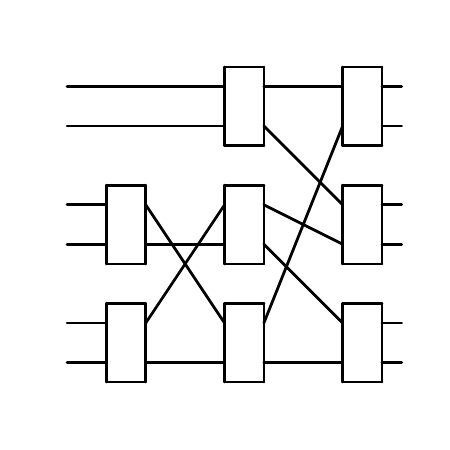
\begin{tikzpicture}[line cap=round,line join=round,>=triangle 45,x=0.5cm,y=0.5cm]
\clip(-2.,-1.) rectangle (8.,9.);

\draw [line width=1.pt] (0.,0.)-- (1.,0.);
\draw [line width=1.pt] (1.,2.)-- (1.,0.);
\draw [line width=1.pt] (1.,2.)-- (0.,2.);
\draw [line width=1.pt] (0.,0.)-- (0.,2.);
\draw [line width=1.pt] (0.,3.)-- (1.,3.);
\draw [line width=1.pt] (1.,3.)-- (1.,5.);
\draw [line width=1.pt] (1.,5.)-- (0.,5.);
\draw [line width=1.pt] (0.,3.)-- (0.,5.);
\draw [line width=1.pt] (3.,8.)-- (3.,6.);
\draw [line width=1.pt] (3.,6.)-- (4.,6.);
\draw [line width=1.pt] (4.,6.)-- (4.,8.);
\draw [line width=1.pt] (4.,8.)-- (3.,8.);
\draw [line width=1.pt] (3.,5.)-- (3.,3.);
\draw [line width=1.pt] (3.,3.)-- (4.,3.);
\draw [line width=1.pt] (4.,3.)-- (4.,5.);
\draw [line width=1.pt] (4.,5.)-- (3.,5.);
\draw [line width=1.pt] (3.,2.)-- (3.,0.);
\draw [line width=1.pt] (3.,0.)-- (4.,0.);
\draw [line width=1.pt] (4.,0.)-- (4.,2.);
\draw [line width=1.pt] (4.,2.)-- (3.,2.);
\draw [line width=1.pt] (6.,8.)-- (6.,6.);
\draw [line width=1.pt] (6.,6.)-- (7.,6.);
\draw [line width=1.pt] (7.,6.)-- (7.,8.);
\draw [line width=1.pt] (7.,8.)-- (6.,8.);
\draw [line width=1.pt] (6.,5.)-- (6.,3.);
\draw [line width=1.pt] (6.,3.)-- (7.,3.);
\draw [line width=1.pt] (7.,3.)-- (7.,5.);
\draw [line width=1.pt] (7.,5.)-- (6.,5.);
\draw [line width=1.pt] (6.,2.)-- (6.,0.);
\draw [line width=1.pt] (6.,0.)-- (7.,0.);
\draw [line width=1.pt] (7.,0.)-- (7.,2.);
\draw [line width=1.pt] (7.,2.)-- (6.,2.);

\draw [line width=1.pt] (0.,4.5)-- (-1.,4.5);
\draw [line width=1.pt] (0.,3.5)-- (-1.,3.5);
\draw [line width=1.pt] (0.,1.5)-- (-1.,1.5);
\draw [line width=1.pt] (0.,0.5)-- (-1.,0.5);
\draw [line width=1.pt] (3.,7.5)-- (-1.,7.5);
\draw [line width=1.pt] (3.,6.5)-- (-1.,6.5);

\draw [line width=1.pt] (1.,4.5)-- (3.,1.5);
\draw [line width=1.pt] (1.,3.5)-- (3.,3.5);
\draw [line width=1.pt] (1.,1.5)-- (3.,4.5);
\draw [line width=1.pt] (1.,0.5)-- (3.,0.5);
\draw [line width=1.pt] (4.,1.5)-- (6.,6.5);
\draw [line width=1.pt] (4.,7.5)-- (6.,7.5);
\draw [line width=1.pt] (4.,6.5)-- (6.,4.5);
\draw [line width=1.pt] (4.,4.5)-- (6.,3.5);
\draw [line width=1.pt] (4.,3.5)-- (6.,1.5);
\draw [line width=1.pt] (4.,0.5)-- (6.,0.5);
\draw [line width=1.pt] (7.,7.5)-- (7.5,7.5);
\draw [line width=1.pt] (7.,6.5)-- (7.5,6.5);
\draw [line width=1.pt] (7.,4.5)-- (7.5,4.5);
\draw [line width=1.pt] (7.,3.5)-- (7.5,3.5);
\draw [line width=1.pt] (7.,1.5)-- (7.5,1.5);
\draw [line width=1.pt] (7.,0.5)-- (7.5,0.5);
\end{tikzpicture}
\end{center}


\todo{antyprzykłady sieci}
\begin{center}
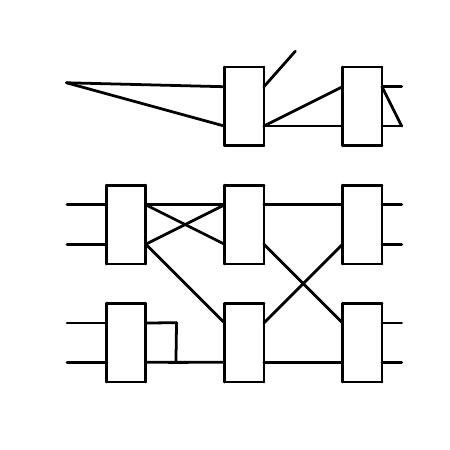
\begin{tikzpicture}[line cap=round,line join=round,>=triangle 45,x=0.5cm,y=0.5cm]
\clip(-2.,-1.) rectangle (8.,9.);
\draw [line width=1.pt] (0.,0.)-- (1.,0.);
\draw [line width=1.pt] (1.,2.)-- (1.,0.);
\draw [line width=1.pt] (1.,2.)-- (0.,2.);
\draw [line width=1.pt] (0.,0.)-- (0.,2.);
\draw [line width=1.pt] (0.,3.)-- (1.,3.);
\draw [line width=1.pt] (1.,3.)-- (1.,5.);
\draw [line width=1.pt] (1.,5.)-- (0.,5.);
\draw [line width=1.pt] (0.,3.)-- (0.,5.);
\draw [line width=1.pt] (3.,8.)-- (3.,6.);
\draw [line width=1.pt] (3.,6.)-- (4.,6.);
\draw [line width=1.pt] (4.,6.)-- (4.,8.);
\draw [line width=1.pt] (4.,8.)-- (3.,8.);
\draw [line width=1.pt] (3.,5.)-- (3.,3.);
\draw [line width=1.pt] (3.,3.)-- (4.,3.);
\draw [line width=1.pt] (4.,3.)-- (4.,5.);
\draw [line width=1.pt] (4.,5.)-- (3.,5.);
\draw [line width=1.pt] (3.,2.)-- (3.,0.);
\draw [line width=1.pt] (3.,0.)-- (4.,0.);
\draw [line width=1.pt] (4.,0.)-- (4.,2.);
\draw [line width=1.pt] (4.,2.)-- (3.,2.);
\draw [line width=1.pt] (6.,8.)-- (6.,6.);
\draw [line width=1.pt] (6.,6.)-- (7.,6.);
\draw [line width=1.pt] (7.,6.)-- (7.,8.);
\draw [line width=1.pt] (7.,8.)-- (6.,8.);
\draw [line width=1.pt] (6.,5.)-- (6.,3.);
\draw [line width=1.pt] (6.,3.)-- (7.,3.);
\draw [line width=1.pt] (7.,3.)-- (7.,5.);
\draw [line width=1.pt] (7.,5.)-- (6.,5.);
\draw [line width=1.pt] (6.,2.)-- (6.,0.);
\draw [line width=1.pt] (6.,0.)-- (7.,0.);
\draw [line width=1.pt] (7.,0.)-- (7.,2.);
\draw [line width=1.pt] (7.,2.)-- (6.,2.);
\draw [line width=1.pt] (0.,4.5)-- (-1.,4.5);
\draw [line width=1.pt] (0.,3.5)-- (-1.,3.5);
\draw [line width=1.pt] (0.,1.5)-- (-1.,1.5);
\draw [line width=1.pt] (0.,0.5)-- (-1.,0.5);
\draw [line width=1.pt] (7.,7.5)-- (7.5,7.5);
\draw [line width=1.pt] (7.,6.5)-- (7.5,6.5);
\draw [line width=1.pt] (7.,4.5)-- (7.5,4.5);
\draw [line width=1.pt] (7.,3.5)-- (7.5,3.5);
\draw [line width=1.pt] (7.,1.5)-- (7.5,1.5);
\draw [line width=1.pt] (7.,0.5)-- (7.5,0.5);
\draw [line width=1.pt] (1.,4.5)-- (3.,4.5);
\draw [line width=1.pt] (1.,4.5)-- (3.,3.5);
\draw [line width=1.pt] (1.,3.5)-- (3.,4.5);
\draw [line width=1.pt] (1.,1.5)-- (1.7813908792453008,1.5039475958137278);
\draw [line width=1.pt] (1.7813908792453008,1.5039475958137278)-- (1.7656781783217494,0.4983347367064437);
\draw [line width=1.pt] (1.7656781783217494,0.4983347367064437)-- (1.,0.5);
\draw [line width=1.pt] (-1.0154698851468411,7.600475554151638)-- (3.,6.5);
\draw [line width=1.pt] (-1.0154698851468411,7.600475554151638)-- (3.,7.5);
\draw [line width=1.pt] (4.,7.5)-- (4.798229456567162,8.401823301252755);
\draw [line width=1.pt] (4.,6.5)-- (6.,7.5);
\draw [line width=1.pt] (4.,6.5)-- (6.,6.5);
\draw [line width=1.pt] (4.,4.5)-- (6.,4.5);
\draw [line width=1.pt] (3.,1.5)-- (1.,3.5);
\draw [line width=1.pt] (3.,0.5)-- (1.7656781783217494,0.4983347367064437);
\draw [line width=1.pt] (4.,3.5)-- (6.,1.5);
\draw [line width=1.pt] (4.,1.5)-- (6.,3.5);
\draw [line width=1.pt] (4.,0.5)-- (6.,0.5);
\draw [line width=1.pt] (7.,7.5)-- (7.5,6.5);
\end{tikzpicture}
\end{center}

\begin{df}
    Mówimy, że sieć przełączników o \(n\) wejściach i \(n\) wyjściach realizuje permutację \(\sigma \in S_n\), gdy każdemu przewodnikowi możemy nadać stan (aktywny lub nieaktywny) tak, by dla sygnałów w kolejności \(0, 1, \ldots, n-1\) na wejściu otrzymać sygnały w kolejności \(\sigma (0), \sigma (1), \ldots, \sigma (n-1)\) na wyjściu. 
\end{df}

\todo{sieć realizująca jakąś małą permutację}

\todo{sieć, która nie może zrealizować jakiejś permutacji}

\begin{df}
    Rozmiar sieci to liczba przełączników w sieci.
\end{df}

\begin{df}
    Głębokość sieci to maksymalna liczba przełączników, przez które przechodzi sygnał od wejścia do wyjścia sieci.  
\end{df}

\todo{sieć o rozmiarze x i głębokości y}
\begin{center}
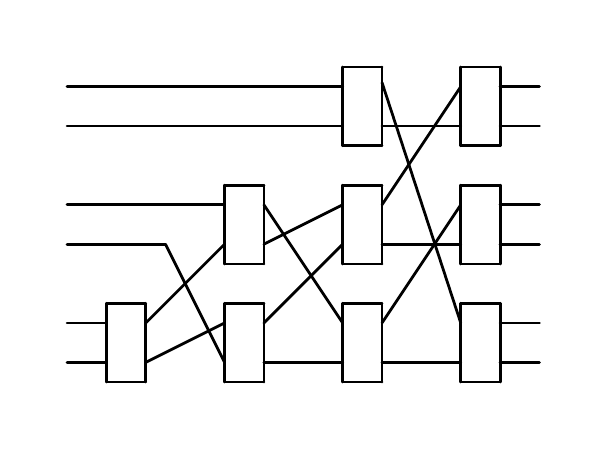
\begin{tikzpicture}[line cap=round,line join=round,>=triangle 45,x=0.5cm,y=0.5cm]

\clip(-2.,-1.) rectangle (12.,9.);
\draw [line width=1.pt] (0.,0.)-- (1.,0.);
\draw [line width=1.pt] (1.,0.)-- (1.,2.);
\draw [line width=1.pt] (1.,2.)-- (0.,2.);
\draw [line width=1.pt] (0.,0.)-- (0.,2.);
\draw [line width=1.pt] (3.,2.)-- (3.,0.);
\draw [line width=1.pt] (4.,0.)-- (3.,0.);
\draw [line width=1.pt] (4.,0.)-- (4.,2.);
\draw [line width=1.pt] (4.,2.)-- (3.,2.);
\draw [line width=1.pt] (6.,2.)-- (6.,0.);
\draw [line width=1.pt] (6.,0.)-- (7.,0.);
\draw [line width=1.pt] (7.,0.)-- (7.,2.);
\draw [line width=1.pt] (7.,2.)-- (6.,2.);
\draw [line width=1.pt] (9.,2.)-- (9.,0.);
\draw [line width=1.pt] (9.,0.)-- (10.,0.);
\draw [line width=1.pt] (10.,0.)-- (10.,2.);
\draw [line width=1.pt] (10.,2.)-- (9.,2.);
\draw [line width=1.pt] (6.,3.)-- (7.,3.);
\draw [line width=1.pt] (7.,3.)-- (7.,5.);
\draw [line width=1.pt] (7.,5.)-- (6.,5.);
\draw [line width=1.pt] (6.,5.)-- (6.,3.);
\draw [line width=1.pt] (9.,3.)-- (10.,3.);
\draw [line width=1.pt] (10.,3.)-- (10.,5.);
\draw [line width=1.pt] (10.,5.)-- (9.,5.);
\draw [line width=1.pt] (9.,5.)-- (9.,3.);
\draw [line width=1.pt] (9.,6.)-- (10.,6.);
\draw [line width=1.pt] (10.,6.)-- (10.,8.);
\draw [line width=1.pt] (10.,8.)-- (9.,8.);
\draw [line width=1.pt] (9.,6.)-- (9.,8.);
\draw [line width=1.pt] (3.,5.)-- (3.,3.);
\draw [line width=1.pt] (4.,3.)-- (3.,3.);
\draw [line width=1.pt] (4.,3.)-- (4.,5.);
\draw [line width=1.pt] (4.,5.)-- (3.,5.);
\draw [line width=1.pt] (6.,6.)-- (7.,6.);
\draw [line width=1.pt] (7.,6.)-- (7.,8.);
\draw [line width=1.pt] (7.,8.)-- (6.,8.);
\draw [line width=1.pt] (6.,8.)-- (6.,6.);
\draw [line width=1.pt] (1.,1.5)-- (3.,3.5);
\draw [line width=1.pt] (3.,4.5)-- (-1.,4.5);
\draw [line width=1.pt] (0.,0.5)-- (-1.,0.5);
\draw [line width=1.pt] (0.,1.5)-- (-1.,1.5);
\draw [line width=1.pt] (1.,0.5)-- (3.,1.5);
\draw [line width=1.pt] (-1.,3.5)-- (1.5,3.5);
\draw [line width=1.pt] (1.5,3.5)-- (3.,0.5);
\draw [line width=1.pt] (6.,6.5)-- (-1.,6.5);
\draw [line width=1.pt] (6.,7.5)-- (-1.,7.5);
\draw [line width=1.pt] (4.,4.5)-- (6.,1.5);
\draw [line width=1.pt] (4.,3.5)-- (6.,4.5);
\draw [line width=1.pt] (4.,1.5)-- (6.,3.5);
\draw [line width=1.pt] (4.,0.5)-- (6.,0.5);
\draw [line width=1.pt] (7.,7.606293605001243)-- (9.,1.5);
\draw [line width=1.pt] (7.,6.5)-- (9.,6.5);
\draw [line width=1.pt] (7.,4.5)-- (9.,7.5);
\draw [line width=1.pt] (7.,3.5)-- (9.,3.5);
\draw [line width=1.pt] (7.,1.5)-- (9.,4.5);
\draw [line width=1.pt] (7.,0.5)-- (9.,0.5);
\draw [line width=1.pt] (10.,1.5)-- (11.,1.5);
\draw [line width=1.pt] (10.,0.5)-- (11.,0.5);
\draw [line width=1.pt] (10.,3.5)-- (11.,3.5);
\draw [line width=1.pt] (10.,4.5)-- (11.,4.5);
\draw [line width=1.pt] (10.,6.5)-- (11.,6.5);
\draw [line width=1.pt] (10.,7.5)-- (11.,7.5);
\end{tikzpicture}
\end{center}

\subsection{Najprostsze sieci}

\begin{pyt}
    Czy istnieje sieć o 6 wejściach i 6 wyjściach mająca rozmiar równy 9, która realizuje wszystkie permutacje z \(S_6\)?
\end{pyt}

Odpowiedź to nie -- łatwo zauważyć, że każdy przełącznik zwiększa liczbę permutacji realizowanych przez sieć co najwyżej dwukrotnie. Wobec tego taka sieć realizuje co najwyżej \(2^9 = 512\) permutacji. Zarazem \(6! = 720 > 512\),  czyli taka sieć nie może istnieć. 

\vspace{1em}

Jakie sieci zatem istnieją? W poniższych rozważaniach pochylimy się nad sieciami głębokości co najwyżej 2 realizującymi identyczność i pewną inną permutację. Konstrukcje tych sieci przeprowadzamy tak, jak autorzy pracy \cite{klo}. Będą one pomocne przy tworzeniu sieci realizującej przesunięcia cykliczne o potęgi 2. 

\begin{lem}\label{lem:perm_symetrie}
    Dla dowolnego \(n\) oraz \(k \in \{0, 1, \ldots, n-1\}\) istnieje sieć o \(n\) wejściach i \(n\) wyjściach o głębokości 1 i rozmiarze co najwyżej \(\floor{\frac n 2}\) realizująca \(\id{n}\) i \(\sym{n}{k}\).
\end{lem}

\begin{proof}
    Ustalmy \(n\) oraz \(k \in \{0, 1, \ldots, n-1\}\). Zauważmy, że 
    \[
    \sym{n}{k} \circ \sym{n}{k} = \id{n} \td
    \]
    Wobec tego permutacja \(\sym n k\) jest inwolucją, a co za tym idzie -- składa się z cykli o rozmiarze co najwyżej 2. Konstrukcja sieci wygląda następująco:
    \begin{itemize}
        \item każdemu cyklowi postaci \((i,j)\) przypisujemy przełącznik, który na wejściach przyjmuje sygnały \(i\) oraz \(j\) z wejścia sieci, a przewody na jego wyjściach prowadzą do wyjść sieci o numerach \(i\) oraz \(j\),
        \item każdemu cyklowi jednoelementowemu postaci \((i)\) przypisujemy przewód biegnący od \(i\)--tego wejścia do \(i\)--tego wyjścia sieci.
    \end{itemize}
    Oczywiście w ten sposób używamy co najwyżej \(\floor{\frac{n}{2}}\) przełączników. 
    Ponadto jeśli wszystkie przełączniki są w stanie nieaktywnym, sieć realizuje \(\id n\), natomiast jeśli wszystkie są w stanie aktywnym, to realizuje \(\sym n k\).
\end{proof}

Zaobserwujmy konstrukcję z lematu \ref{lem:perm_symetrie} dla \(n=4\) i \(k=2\).

\todo{rysunek sieci}

Lemat \ref{lem:perm_symetrie} można jednak uogólnić -- zauważmy, że nie korzystamy z żadnych własności symetrii, poza tym, że \( \sym n k \circ \sym n k = \id n \).

\begin{lem}\label{lem:perm_inwolucje}
    Dla dowolnego \(n\) oraz \(\sigma \in S_n\), które jest inwolucją (to znaczy \(\sigma \circ \sigma = \id n\)) istnieje sieć o \(n\) wejściach i \(n\) wyjściach o głębokości 1 i rozmiarze co najwyżej \(\floor{\frac{n}{2}}\) realizująca \(\id n\) oraz \(\sigma\).
\end{lem}

\begin{proof}
    Konstrukcja jest identyczna jak ta w lemacie \ref{lem:perm_symetrie}.
\end{proof}

\begin{lem}\label{lem:perm_shifty}
     Dla dowolnego \(n\) oraz \(k \in \{0, 1, \ldots, n-1\}\) istnieje sieć o \(n\) wejściach i \(n\) wyjściach o głębokości 2 realizująca \(\id n\) i \(\shift{n}{k}\).
\end{lem}

\begin{proof}
    Ustalmy \(n\). Zauważmy, że
    \[
    \sym n k (\sym n 0 (i)) = \sym n k (-i \mod n) = (k - (-i)) \mod n = (k + i) \mod n  = \shift n k (i)
    \]
    dla każdego \(i \in \{0, 1, \ldots, n-1\}\). Wobec tego \(\shift n k = \sym n k \circ \sym n 0\). Stwórzmy zatem sieć przełączników o dwóch warstwach -- pierwsza z nich niech będzie siecią realizującą \(\id n\) i \(\sym n 0\), a druga siecią realizującą \(\id n\) i  \(\sym n k\) (jak w lemacie \ref{lem:perm_symetrie}). Taka sieć ma głębokość 2. Jeśli wszystkie przełączniki są nieaktywne, to realizuje \(\id n\), natomiast jeśli wszystkie są aktywne, to z powyższego rachunku wynika, że realizuje \(\shift n k\).
\end{proof}

\todo{przykład konstrukcji}

\begin{lem}
    Dla dowolnego \(n\) oraz \(\sigma \in S_n\) istnieje sieć o  \(n\) wejściach i \(n\) wyjściach o głębokości 2 realizująca \(\id n\) i \(\sigma\).
\end{lem}

\begin{proof}
    Ustalmy \(n\) oraz \(\sigma \in S_n\). Oczywiście \(\sigma\) może być przedstawiona jako złożenie cykli rozłącznych:
    \[
        \sigma = \sigma_1 \circ \sigma_2 \circ \ldots \circ \sigma_k \td
    \]
    Prostą konsekwencją lematu \ref{lem:perm_shifty} jest to, że istnieje sieć o głębokości 2, która realizuje \(\id n\) oraz \(\sigma_i\) dla każdego \(i\). Konstrukcja sieci żądanej w tym lemacie polega na złożeniu tych sieci dla każdego \(\sigma_i\). Z rozłączności cykli wynika, że będzie miała ona głębokość równą 2. 
\end{proof}



% ---------- sieć Beneša-Waksmana -----------------

\section{Sieć Beneša--Waksmana}

\begin{pyt}
    Czy istnieje sięć realizująca wszyskie permutacje z \(S_n\)?
\end{pyt}
Odpowiedź to tak.
\todo{Przykład jak konstruować nie optymalnie sieci permutacji}
\begin{pyt}
    Jaka jest minimalna liczba przełączników żeby zrealizować wszystkie permutacje z \(S_n\)?
\end{pyt}
\begin{tw}
    Żeby zrealizować każdą permutację z \(S_n\) potrzeba sieci o co najmniej \(\Omega(n \log n )\) przełącznikach.
\end{tw}
\begin{proof}
Ustalmy n $\in \mathbb{N}$.
Zauważmy, że przełącznik, co najwyżej, zwiększa ilość realizowanych permutacji dwukrotnie.
Niech $\sigma$ będzie siecią która realizuje wszystkie \(n!\) permutacji. Niech \(F\) będzie funkcją która sieci przyporządkowuje ilość przełączników która się w niej znajduje.
Wtedy $log(n!) \leq F(\sigma)$. Ze wzoru Stirlinga z możemy oszacować \(n!\) z dołu przez $(n/e)^n$. Wówczas
\[
    \log (n!) \geq \log ( (n/e)^n ) = n(\log n - \log e) = \Omega(n \log n)
\]
\end{proof}
\begin{pyt}
    Jak skonstruować taką sieć?
\end{pyt}
Dla uproszczenia przyjmiemy, że \(n = 2^k\) dla pewnego \(k \in \mathbb{N}\).
Konstrukcja polega na podzieleniu problemu na dwa identyczne pod problemy i pomysłowym połączeniu tych dwóch pod problemów w pełne rozwiązanie.
Na wejściu mamy \(n\) przełączników z każdego ich wyjścia prowadzimy przewód do wejść obu pod sieci o rozmiarze \(n/2\).
Podobnie na wyjściu mamy \(n\) przełączników i z każdego ich wejścia prowadzimy przewód do wyjść obu podsieci o rozmiarze \(n/2\).
\todo{Konstrukcja sieci Beneša--Waksmana}
\begin{center}
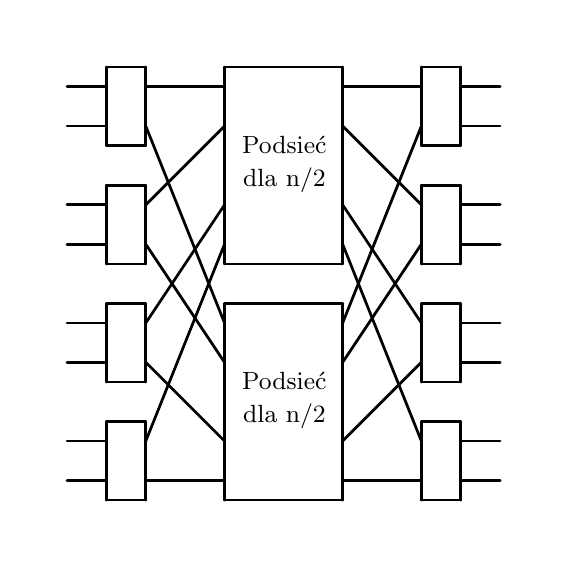
\begin{tikzpicture}[line cap=round,line join=round,>=triangle 45,x=0.5cm,y=0.5cm]
\clip(-2.,-1.) rectangle (11.,12.);
\draw [line width=1.pt] (0.,0.)-- (1.,0.);
\draw [line width=1.pt] (1.,0.)-- (1.,2.);
\draw [line width=1.pt] (1.,2.)-- (0.,2.);
\draw [line width=1.pt] (0.,2.)-- (0.,0.);
\draw [line width=1.pt] (0.,3.)-- (1.,3.);
\draw [line width=1.pt] (1.,3.)-- (1.,5.);
\draw [line width=1.pt] (1.,5.)-- (0.,5.);
\draw [line width=1.pt] (0.,5.)-- (0.,3.);
\draw [line width=1.pt] (0.,6.)-- (1.,6.);
\draw [line width=1.pt] (1.,6.)-- (1.,8.);
\draw [line width=1.pt] (1.,8.)-- (0.,8.);
\draw [line width=1.pt] (0.,8.)-- (0.,6.);
\draw [line width=1.pt] (0.,9.)-- (1.,9.);
\draw [line width=1.pt] (1.,9.)-- (1.,11.);
\draw [line width=1.pt] (1.,11.)-- (0.,11.);
\draw [line width=1.pt] (0.,11.)-- (0.,9.);
\draw [line width=1.pt] (3.,11.)-- (3.,6.);
\draw [line width=1.pt] (3.,6.)-- (6.,6.);
\draw [line width=1.pt] (6.,11.)-- (6.,6.);
\draw [line width=1.pt] (6.,11.)-- (3.,11.);
\draw [line width=1.pt] (3.,5.)-- (3.,0.);
\draw [line width=1.pt] (3.,5.)-- (6.,5.);
\draw [line width=1.pt] (6.,5.)-- (6.,0.);
\draw [line width=1.pt] (6.,0.)-- (3.,0.);
\draw [line width=1.pt] (8.,11.)-- (9.,11.);
\draw [line width=1.pt] (9.,11.)-- (9.,9.);
\draw [line width=1.pt] (9.,9.)-- (8.,9.);
\draw [line width=1.pt] (8.,9.)-- (8.,11.);
\draw [line width=1.pt] (8.,8.)-- (8.,6.);
\draw [line width=1.pt] (8.,6.)-- (9.,6.);
\draw [line width=1.pt] (9.,6.)-- (9.,8.);
\draw [line width=1.pt] (9.,8.)-- (8.,8.);
\draw [line width=1.pt] (8.,5.)-- (8.,3.);
\draw [line width=1.pt] (8.,3.)-- (9.,3.);
\draw [line width=1.pt] (9.,3.)-- (9.,5.);
\draw [line width=1.pt] (9.,5.)-- (8.,5.);
\draw [line width=1.pt] (8.,2.)-- (8.,0.);
\draw [line width=1.pt] (8.,0.)-- (9.,0.);
\draw [line width=1.pt] (9.,0.)-- (9.,2.);
\draw [line width=1.pt] (9.,2.)-- (8.,2.);
\draw [line width=1.pt] (0.,10.5)-- (-1.,10.5);
\draw [line width=1.pt] (0.,9.5)-- (-1.,9.5);
\draw [line width=1.pt] (0.,7.5)-- (-1.,7.5);
\draw [line width=1.pt] (0.,6.5)-- (-1.,6.5);
\draw [line width=1.pt] (0.,4.5)-- (-1.,4.5);
\draw [line width=1.pt] (0.,3.5)-- (-1.,3.5);
\draw [line width=1.pt] (0.,1.5)-- (-1.,1.5);
\draw [line width=1.pt] (0.,0.5)-- (-1.,0.5);
\draw [line width=1.pt] (1.,10.5)-- (3.,10.5);
\draw [line width=1.pt] (1.,9.5)-- (3.,4.5);
\draw [line width=1.pt] (1.,7.5)-- (3.,9.5);
\draw [line width=1.pt] (1.,6.5)-- (3.,3.5);
\draw [line width=1.pt] (1.,4.5)-- (3.,7.5);
\draw [line width=1.pt] (1.,3.5)-- (3.,1.5);
\draw [line width=1.pt] (1.,1.5)-- (3.,6.5);
\draw [line width=1.pt] (1.,0.5)-- (3.,0.5);
\draw [line width=1.pt] (6.,10.5)-- (8.,10.5);
\draw [line width=1.pt] (8.,9.5)-- (6.,4.5);
\draw [line width=1.pt] (8.,7.5)-- (6.,9.5);
\draw [line width=1.pt] (8.,6.5)-- (6.,3.5);
\draw [line width=1.pt] (8.,4.5)-- (6.,7.5);
\draw [line width=1.pt] (8.,3.5)-- (6.,1.5);
\draw [line width=1.pt] (8.,1.5)-- (6.,6.5);
\draw [line width=1.pt] (8.,0.5)-- (6.,0.5);
\draw [line width=1.pt] (9.,10.5)-- (10.,10.5);
\draw [line width=1.pt] (9.,9.5)-- (10.,9.5);
\draw [line width=1.pt] (9.,7.5)-- (10.,7.5);
\draw [line width=1.pt] (9.,6.5)-- (10.,6.5);
\draw [line width=1.pt] (9.,4.5)-- (10.,4.5);
\draw [line width=1.pt] (9.,3.5)-- (10.,3.5);
\draw [line width=1.pt] (9.,1.5)-- (10.,1.5);
\draw [line width=1.pt] (9.,0.5)-- (10.,0.5);

\draw (3.2,9.5) node[anchor=north west, align=center] {\small Podsieć \\ \small dla n/2};
\draw (3.2,3.5) node[anchor=north west, align=center] {\small Podsieć \\ \small dla n/2};
\end{tikzpicture}
\end{center}


\begin{tw}
    Sieć Beneša--Waksmana realizuje wszystkie permutacje.
\end{tw}
\begin{proof}
    Niech $\pi$ będzie dowolną permutacją z $S_n$. Pokażemy, że istnieje ustawienie przełączników takie, że dane z i tego portu wejściowego zostaną przesłane na $\pi(i)$ port wyjściowy. 
    Niech $G_\pi = (V, E)$ będzie grafem w którym:
    \begin{itemize}
        \item $V = V_i \cup V_o \cup V_m$. Każdy z tych wierzchołków otrzymuje etykietę.
        \begin{itemize}
            \item $V_i$ wierzchołki odpowiadające portom wejściowym sieci.
             Wierzchołek z $V_i$ odpowiadający i-temu portowi wejściowemu otrzymuje etykietę i.
            \item $V_o$ wierzchołki odpowiadające portom z ostatniej warstwy po dwa na przełącznik. Jeżeli te wierzchołki odpowiadają j-temu przełącznikowi z ostatniej warstwy to otrzymują etykiety $i''$ i $k''$ takie, że $2 - 1 = \pi(i)$ oraz $2j = \pi(k)$.
            \item $V_m$ dodatkowe wierzchołki które otrzymują etykiety ze zbioru ${1', 2', ..., n'}$
        \end{itemize}
        \item $E = E_i \cup E_m \cup E_o$ składa się z:
        \begin{itemize}
            \item $n/2$ krawędzi w zbiorze $E_i$ o etykietach $2i-1$ i $2i$, a więc takie które odpowiadają sąsiednim portom wejściowym.
            \item $n/2$ krawędzi w zbiorze $E_o$ łączący wierzchołki odpowiadające temu samemu przełącznikowi na ostatniej warstwie.
            \item  $2n$ krawędzi w zbiorze $E_m$ łączących wierzchołki o etykietach $i$ i $i'$ oraz wierzchołki o etykietach $i'$ i $i''$.
        \end{itemize}
    \end{itemize} 
    Tak zdefiniowany graf jest sumą rozłączoną cykli parzystej długości. Jest tak ponieważ stopień każdego wierzchołka jest równy 2 a więc jest sumą rozłącznych cykli. Każdy cykl zawiera parzystą liczbę wierzchołków z $V_i$ i $V_o$ z czego wynika, że zawiera też parzystą liczbę wierzchołków z $V_m$.
    Wobec tego graf $G_\pi$ jest dwu kolorowalny.
    W związku z tym takie kolorowanie spełnia:
    \begin{itemize}
        \item Wierzchołki odpowiadające sąsiednim portom otrzymują różne kolory.
        \item Wierzchołki o etykietach $i$ oraz $i''$ otrzymują ten sam kolor
    \end{itemize}
    Konsekwencja tego jest, że jeżeli:
    \begin{itemize}
        \item Dane z białych portów wejściowych wyślemy do górnej podsieci, a czarne do dolnej. 
        \item Ustawiamy elementy w górnej i dolnej podsieci tak żeby per-mutowały zgodnie z permutacją $\pi$.
        \item W ostatniej warstwie dla j-tego przełącznika i odpowiadającej mu etykiecie białego wierzchołka i oraz czarnemu wierzchołkowi, o etykiecie k, na tym samym przełączniku. Stosujemy regułę która mówi: Jeśli $i = \pi(2j - 1)$ oraz $k = \pi(2j)$ to przełącznik jest w stanie nieaktywnym w przeciwnym wypadku jest w stanie aktywnym.
    \end{itemize}

\end{proof}
\todo{obrazek do dwukolorowania}
\todo{Przykład małej sieci}

\begin{pyt}
    Czy da się lepiej?
\end{pyt}
Tak. Można usunąć po jednym przełączniku na każdym poziomie sieci.
\begin{proof}
    Zauważmy, że jeżeli ustalimy kolor jednego z wierzchołków odpowiadającym portom wyjściowym to jednoznacznie ustalimy całe dwu kolorowanie. Wtedy możemy usunąć przełącznik na którym ustawiliśmy kolor. Ponieważ w białej podsieci istnieje tak ustawienie przełączników, która odpowiada permutacji białych przełączników. 
\end{proof}

% --- Sieć realizująca wszystkie przesunięcia cykliczne ---

\section{Sieć realizująca wszystkie przesunięcia cykliczne}

% -- Sieć realizująca przesunięcia cykliczne o potęgi 2 ---

\section{Sieć realizująca przesunięcia cykliczne o potęgi 2}

W tym rozdziale chcemy zastanowić się nad konstrukcją sieci o \(n\) wejściach i \(n\) wyjściach realizującej przesunięcia cykliczne o potęgi 2 nie większe niż \(n\), to znaczy chcemy zrealizować zbiór

\[
\twoshift{n} = \{ \id n \tc \shift n {2^0} \tc \shift n {2^1} \tc \ldots \shift n {2^l}\} \tc
\]

gdzie \(2^l \leq n\) oraz \(2^{l+1} > n\). Dla uproszczenia przyjmiemy, że \(n = 2^{2^r}\) dla pewnego \(r \in \N\) i oznaczymy \( m = \sqrt{n} = 2^{2^{r-1}} \). Uogólnienie konstrukcji dla dowolnego \(n \in \N\) zostało przedstawione w \cite{klo}.

\vspace{1em}

W tym rozdziale będziemy wyobrażać sobie zbiór \(\{0, 1, 2, \ldots, n-1\}\) jako macierz o wymiarach \(m \times m\) -- to uzasadnia wybór \(n\), które jest kwadratem liczby naturalnej. Na przykład dla \(r = 2\) mamy \(n = 2^{2^2} = 2^4 = 16\), a macierzowa reprezentacja zbioru wygląda następująco:
\[
\begin{matrix}
 0 &  1 &  2 &  3 \\
 4 &  5 &  6 &  7 \\
 8 &  9 & 10 & 11 \\
12 & 13 & 14 & 15
\end{matrix}
\]

Zastanówmy się teraz, jak wyglądają przesunięcia cykliczne o \(2^k\) w tej reprezentacji. Gdy \(2^k\) jest \textit{duże}, to znaczy \(2^k \geq m\) (równoważnie \(k \geq 2^{r-1}\)), to \(m \, | \, 2^k\). Wobec tego \(\shift n {2^k}\) jest przesunięciem cyklicznym o \(2^k / m = 2^k / 2^{2^{r-1}} = 2^{k - 2^{r-1}}\) na zbiorze wierszy. Na przykład dla \(n = 64 = 2^{2^3}\) oraz \(2^k = 2^4 = 2 \cdot \sqrt{64}\) mamy

\vspace{0.5em}

\begin{minipage}{.5\textwidth} %

\[
\begin{matrix}
 0 &  1 &  2 &  \ldots & 7 \\
 8 &  9 & 10 &  \ldots & 15 \\
\ldots & & \ddots &  & \vdots \\
48 & 49 & 50 & \ldots & 55 \\
56 & 57 & 58 & \ldots & 63 
\end{matrix}
\]

\begin{center} \it
    Zbiór przed wykonaniem \(\shift {64} {16}\).
\end{center}

\end{minipage} %
\begin{minipage}{.5\textwidth} %

\[
\begin{matrix}
16 & 17 & 18 & \ldots & 23 \\
24 & 25 & 26 & \ldots & 31 \\
\ldots & & \ddots &  & \vdots \\
56 & 57 & 58 & \ldots & 63 \\
0 &  1 &  2 &  \ldots & 7 \\
8 &  9 & 10 &  \ldots & 15 \\
\end{matrix}
\]

\begin{center} \it
    Zbiór po wykonaniu \(\shift {64} {16}\).
\end{center}
\end{minipage}

\vspace{1em}

Możemy także pomyśleć o tym nieco inaczej. Dokładniej, \(\shift n {2^k}\) może być wykonany w 3 etapach:

\begin{enumerate}
    \item transpozycja macierzy,
    \item \(\shift {m} {2^k/m}\) na wierszach tak otrzymanej macierzy,
    \item transpozycja macierzy.
\end{enumerate}

Przeanalizujmy to na powyższym przykładzie -- \(n = 64\) oraz \(2^k = 16\).

\vspace{0.5em}

\begin{minipage}{.5\textwidth} %

\[
\begin{matrix}
 0 &  1 &  2 &  \ldots & 7 \\
 8 &  9 & 10 &  \ldots & 15 \\
\ldots & & \ddots &  & \vdots \\
48 & 49 & 50 & \ldots & 55 \\
56 & 57 & 58 & \ldots & 63 
\end{matrix}
\]

\begin{center} \it
    Początkowy zbiór.
\end{center}

\end{minipage} %
\begin{minipage}{.5\textwidth} %

\[
\begin{matrix}
 0 &  8 &  16 &  \ldots & 56 \\
 1 &  9 &  17 &  \ldots & 57 \\
\ldots  & & \ddots &     & \vdots \\
 6 & 14 & 22 & \ldots   & 62 \\
 7 & 15 & 23 & \ldots   & 63 
\end{matrix}
\]

\begin{center} \it
    Zbiór po wykonaniu transpozycji.
\end{center}
\end{minipage}

\vspace{0.5em}

\begin{minipage}{.5\textwidth} %
\[
\begin{matrix}
 16 &  24 &  \ldots & 0 & 8 \\
 17 &  25 &  \ldots & 1 & 9 \\
\ldots  & &  \ddots &   & \vdots \\
 22 &  30 &  \ldots & 6 & 14 \\
 23 &  31 &  \ldots & 7 & 15
\end{matrix}
\]

\begin{center} \it
    Zbiór po wykonaniu \(\shift{8}{2}\) na wierszach macierzy.
\end{center}

\end{minipage} %
\begin{minipage}{.5\textwidth} %

\[
\begin{matrix}
 16 &  17 &  \ldots & 22 & 23 \\
 24 &  25 &  \ldots & 30 & 31 \\
\ldots  & &  \ddots &    & \vdots \\
  0 &   1 &  \ldots &  6 & 7 \\
  8 &   9 &  \ldots &  14 & 15
\end{matrix}
\]

\begin{center} \it
    Zbiór po wykonaniu transpozycji.
\end{center}
\end{minipage}

Co się dzieje, gdy \(2^k\) jest \textit{małe} (to znaczy \(2^k < m \))? Wtedy zmiany w układzie liczb zachodzą także wewnątrz wierszy. Istotnie -- \(\shift n {2^k}\) możemy wówczas przedstawić jako dwa etapy:
\begin{enumerate}
    \item \(\shift{m}{2^k}\) wewnątrz każdego wiersza,
    \item \(\shift{m}{1}\) wewnątrz ostatnich \(2^k\) kolumn.
\end{enumerate}

Przyjrzyjmy się tym etapom na przykładzie -- niech \(n=64\) oraz \(2^k = 2\).

\vspace{0.5em}

\begin{minipage}{.5\textwidth} %

\[
\begin{matrix}
 0 &  1 &  2 &  \ldots & 7 \\
 8 &  9 & 10 &  \ldots & 15 \\
\ldots & & \ddots &  & \vdots \\
48 & 49 & 50 & \ldots & 55 \\
56 & 57 & 58 & \ldots & 63 
\end{matrix}
\]

\begin{center} \it
    Początkowy zbiór.
\end{center}

\end{minipage} %
\begin{minipage}{.5\textwidth} %

\[
\begin{matrix}
 2  &  3 & \ldots &  0 &  1 \\
 10 & 11 & \ldots &  8 &  9 \\
\ldots & & \ddots &  & \vdots \\
 50 & 51 & \ldots & 48 & 49 \\
 58 & 59 & \ldots & 56 & 57 \\ 
\end{matrix}
\]

\begin{center} \it
    Zbiór po wykonaniu \(\shift 8 2\) na każdym wierszu.
\end{center}
\end{minipage}

\vspace{1em}

\begin{minipage}{.5\textwidth} %

\[
\begin{array}{c c  c c}
 2  &  3 & \ldots & 7 \\
 10 & 11 & \ldots & 15 \\
\ldots & & \ddots &  \vdots \\
 50 & 51 & \ldots & 56  \\
 58 & 59 & \ldots & 63  \\ 
\end{array}
\begin{array}{| c c |}
\hline
 0 &  1 \\
 8 &  9 \\
\vdots & \vdots \\
 48 & 49 \\
 56 & 57 \\
 \hline
\end{array}
\]

\begin{center} \it
    Kolumny, na których należy wykonać \(\shift 8 1\).
\end{center}
\end{minipage}
\begin{minipage}{.5\textwidth} %

\[
\begin{matrix}
 2  &  3 & \ldots & 8  &  9  \\
 10 & 11 & \ldots & 16 & 17\\
\ldots & & \ddots &  & \vdots \\
 50 & 51 & \ldots & 56 & 57 \\
 58 & 59 & \ldots & 0 &  1 \\ 
\end{matrix}
\]

\begin{center} \it
    Zbiór po wykonaniu \(\shift 8 1\) na 2 ostatnich kolumnach.
\end{center}
\end{minipage}

\vspace{1em}

Podsumowując, przesunięcia cykliczne o \(2^k\) realizujemy w następujący sposób:

\begin{itemize}
    \item gdy \(2^k\) jest małe, wykonujemy \(\shift{m}{2^k}\) wewnątrz każdego wiersza, a następnie \(\shift{m}{1}\) wewnątrz ostatnich \(2^k\) kolumn,
    \item gdy \(2^k\) jest duże, transponujemy macierz, wykonujemy \(\shift {m} {2^k/m} \) na wierszach i znowu transponujemy macierz.
\end{itemize}

To pozwala już sformułować przybliżoną konstrukcję sieci. Aby skonstruować \(P_n\) -- sieć realizującą \(\twoshift n\), potrzebujemy następujących podsieci (zwanych dalej \textit{blokami}):

\begin{itemize}
    \item sieci realizującej transpozycję i \(\id n\) (oznaczmy ją \(T_1\)),
    \item \(m\) sieci realizujących \( \twoshift m\) -- czyli \(m\) kopii sieci \(P_m\) (nazwijmy je \textit{blokiem wierszowym}),
    \item \(m\) sieci realizujących \(\shift m 1\) oraz \(\id m\) dla każdej kolumny, takich jak w lemacie \ref{lem:perm_shifty} -- nazwijmy je \textit{blokiem kolumnowym}
    \item oraz drugiej sieci realizującej transpozycję i \(\id n\) (oznaczmy ją \(T_2\)).
\end{itemize}

\todo{schematyczny rysunek bloków}

Oczywiście transpozycja jest inwolucją -- w związku z tym sieci \(T_1\) i \(T_2\) mogą zostać utworzone tak jak w lemacie \ref{lem:perm_inwolucje}. 
W terminach tak skonstruowanej sieci zrealizowanie przesunięcia cyklicznego o \(2^k\) wygląda następująco:

\begin{itemize}
    \item gdy \(2^k\) jest małe, aktywujemy blok wierszowy, tak by wykonał \(\shift m {2^k}\) na każdym wierszu, a następnie aktywujemy blok kolumnowy, tak by wykonał \(\shift m 1\) na ostatnich \(2^k\) kolumnach,
    \item gdy \(2^k\) jest duże, aktywujemy sieć \(T_1\), tak by wykonała transpozycję, aktywujemy blok wierszowy, tak by wykonał \(\shift m {2^k/m}\) na każdym wierszu, a na końcu aktywujemy aktywujemy sieć \(T_2\), tak by wykonała transpozycję.
\end{itemize}

Udało nam się skonstruwać sieć realizującą \(\twoshift n\). Zbadajmy teraz jej głębokość i rozmiar.

\begin{lem}
    Sieć przedstawiona wyżej ma głębokość równą \(D(n) = \Theta(\log \log n)\).
\end{lem}

\begin{proof}
    Zauważmy, że zarówno blok \(T_1\), jaki i blok \(T_2\), mają głębokość równą 1. Blok kolumnowy ma głębokość równą 2, a blok wierszowy -- \(D(m) = D(\sqrt{n})\). Wobec tego głębokość sieci wyraża się następującym równaniem rekurencyjnym:
    \[
    D(n) = D(\sqrt n) + O(1) \td
    \]
    Do rozwiązania tej rekurencji zastosujemy metodę podstawiania. Niech \(s = \log n\). Mamy wówczas
    \[
    D(2^s) = D(2^{s/2}) + O(1) \td
    \]
    Oznaczmy \(B(s) = D(2^s)\). Dla \(B\) rekurencja przedstawia się następująco:
    \[
    B(s) = B\left(\frac s 2\right) + O(1) \td
    \]
    Na mocy twierdzenia o rekurencji uniwersalnej (ang. \textit{master theorem}, \cite{cormen}) otrzymujemy
    \[
    B(s) = \Theta(\log s) \tc
    \]
    a zapisując powyższą równość w terminach \(D\), dostajemy
    \[
    D(n) = D(2^s) = B(s) = \Theta(\log s) = \Theta(\log \log n) \td
    \]
\end{proof}

\begin{lem}
    Sieć przedstawiona wyżej ma rozmiar równy \(S(n) = \Theta(n \log \log n)\). 
\end{lem}

\begin{proof}
    Zauważmy, że sieci \(T_1\) i \(T_2\) mają rozmiar równy \( \floor{\frac{n - \sqrt{n}}{2}} \). Ponadto rozmiar całego bloku kolumnowego wynosi co najwyżej \(m \cdot \frac{m}{2} \cdot 2\), gdzie \(m = \sqrt{n}\), a rozmiar bloku wierszowego to \(mS(m)\).  Otrzymujemy zatem następujące równanie rekurencyjne
    \[
    S(n) = 2 \cdot \floor{\frac{n - \sqrt{n}}{2}} + O\left(\sqrt{n} \cdot \frac{\sqrt{n}}{2} \cdot 2\right) + \sqrt{n}S(\sqrt{n})
    = \sqrt{n}S(\sqrt{n}) + \Theta(n) \td
    \]
    Przypomnijmy, że \(n = 2^{2^r}\). 
    % Przeprowadzimy dowód indukcyjny względem \(r\). Załóżmy, że 
    % \[
    % S(\sqrt n) = S\lt( 2^{2^{r-1}} \rt) = \Theta\lt( 2^{2^{r-1}} (r-1)\rt) \tc
    % \]
    % czyli istnieją \(c, d \in \R_{+}\), takie że
    % \[
    % c \cdot 2^{2^{r-1}} (r-1)  \leq S\lt( 2^{2^{r-1}} \rt) \leq
    % d \cdot 2^{2^{r-1}} (r-1) \td
    % \]
    % Wobec tego
    % \begin{align*}
    %     S\lt( 2^{2^r} \rt) 
    %     &= 2^{2^{r-1}} \cdot S\lt( 2^{2^{r-1}} \rt) + \Theta\lt( 2^{2^r} \rt) \\
    %     &\geq  2^{2^{r-1}} \cdot c \cdot 2^{2^{r-1}} (r-1) +  \Theta\lt( 2^{2^r} \rt) \\
    %     &= c \cdot 2^{2^r} (r-1) + \Theta\lt( 2^{2^r} \rt) \\
    %     &= c \cdot 2^{2^r} r - c \cdot 2^{2^r} +  \Theta\lt( 2^{2^r} \rt) \\
    %     &\geq c \cdot 2^{2^r} r
    % \end{align*}

    % Mamy zatem
    % \begin{align*}
    %     S(n) &= S(2^{2^r}) = 2^{2^{r-1}} \cdot S\left( 2^{2^r-1} \right) + O\lt( 2^{2^r} \rt) \\
    %     &= 2^{2^{r-1}} \cdot \lt( 2^{2^{r-2}} \cdot S\left( 2^{2^r-2} \right) + O\lt( 2^{2^{r-1}} \rt) \rt) + O\lt( 2^{2^r} \rt) \\
    %     &= 2^{2^{r-1} + 2^{r-2}} \cdot S \lt( 2^{2^{r-2}} \rt) + 2^{2^{r-1}} \cdot O\lt( 2^{2^{r-1}} \rt) + O\lt( 2^{2^{r}} \rt)
    % \end{align*}
    \todo{dokończyć dowód}
    
\end{proof}


% ------------------ Co dalej? -------------------

\section{Co dalej?}

Losowe ustawianie przełączników -- analiza probabilistyczna. 

% ------------- bibliografia ----------------------

\begin{thebibliography}{9}
\bibitem{klo}
Juraj Hromkovič, Przemyslawa Kanarek, Ralf Klasing, Krzysztof Lorys, Walter Unger, et al.. \emph{On the Size of Permutation Networks and Consequences for Efficient Simulation of Hypercube Algorithms on Bounded-Degree Networks}. SIAM Journal on Discrete Mathematics, 2009, 23 (3), pp.1612–1645. ff10.1137/060669164ff. ffhal-00402764f

\bibitem{cormen}
Thomas H. Cormen, Charles E. Leiserson, Ronald L. Rivest, Clifford Stein, \emph{Introduction to Algorithms}, The MIT Press, 2022
\end{thebibliography}

\end{document}